\subsection{fstatat}
前面的stat是通过fd去获得stat状态,而相比于fstat,fstatat可以通过路径名来定位文件,而不仅仅依赖文件描述符来获取文件信息。
本小节将重点介绍\textbf{fstatat系统调用相较于fstat不同的地方},因此会忽略部分与fstat相同或类似的算法部分。

\subsubsection{系统调用原型}
\begin{lstlisting}[language={Rust},
	caption={os/src/syscall/fs.rs}]
    pub fn sys_fstatat(dirfd: usize, path: *const u8, buf: *mut u8, flags: u32);
\end{lstlisting}
参数解释:\\
dirfd:用于定位文件的目录文件描述符(file descriptor)。它可以是当前工作目录的文件描述符,也可以是其它目录的文件描述符。\\
path:文件的路径名。它可以是绝对路径或相对路径。\\
buf:一个指向stat结构的指针,用于接收文件详细信息。\\
flags:一些标记选项,控制fstatat的行为。\\
在NPUcore中,flags有如下几种类型:
\begin{lstlisting}[language={Rust},
	caption={NPUcore中的fstatat~flags选项}]
pub struct FstatatFlags: u32 {
        const AT_EMPTY_PATH = 0x1000; \\允许空路径名(仅用于目录文件)
        const AT_NO_AUTOMOUNT = 0x800; \\禁止系统自动挂载文件系统
        const AT_SYMLINK_NOFOLLOW = 0x100; \\不跟随符号链接
    }
\end{lstlisting}
\subsubsection{fstatat流程}
fstatat函数相较于fstat多了两个阶段。第一是根据Flags查找并获取当前的fstatat标记选项,第二是以只读模式打开dirfd所指向的file_descriptor,如果可以正常打开,再拷贝stat状态至buffer。
为此我们需要在fstat的流程图中添加部分流程框。
\begin{figure}[H]
    \centering
    \scalebox{0.13}{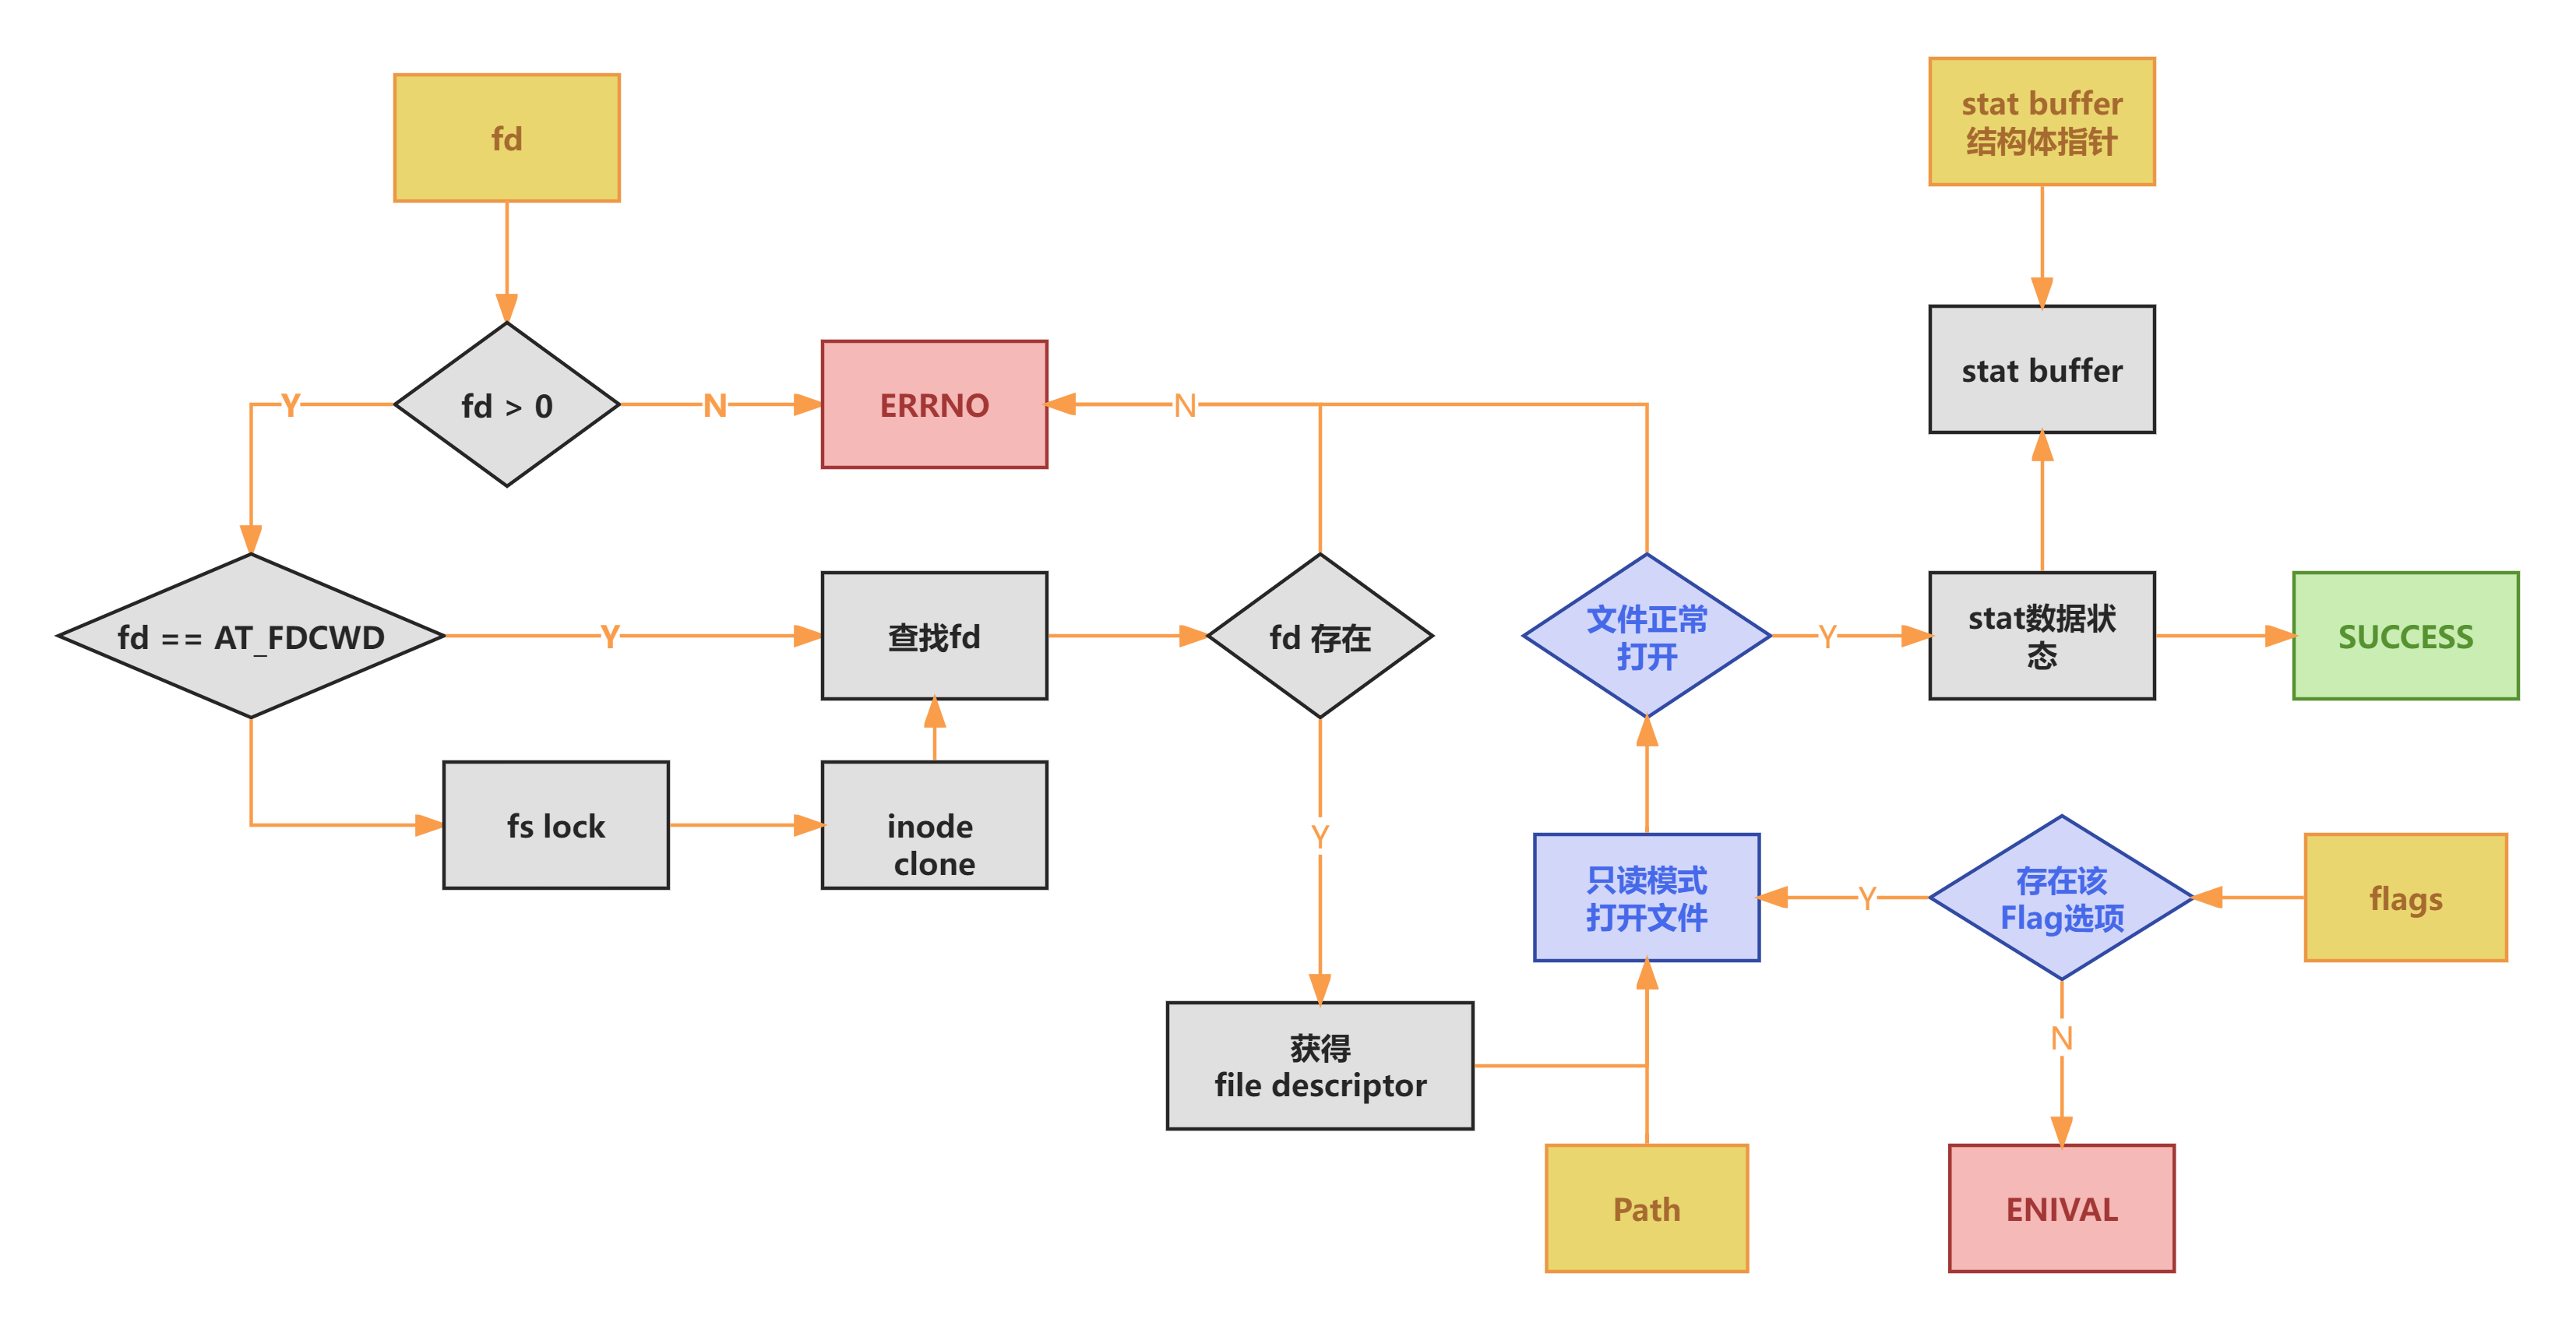
\includegraphics{figures/09-04-fstatat-流程图.png}}
    \caption{fstatat流程框图,灰色框代表与fstat重复部分,黄色框代表输入,红色与绿色框分别是两种不同的输出,靛蓝色框代表与fstat不同的流程。}
\end{figure}
\subsubsection{fstatat代码详解}
由于fstatat与fstat耦合代码较多,这里只涉及fstatat独有的部分代码。
第一个不同是获取Flag部分。
1.首先,通过match语句将flags值转换为FstatatFlags类型的枚举值。
2.将FstatatFlags的flags值转换为FstatatFlags枚举类型的标志位。如果转换成功(Some(flags)),则将转换后的枚举值赋给flags变量。如果转换失败(None),则执行下面的代码块。
3.在代码块中,打印一个警告信息(warn!("[sys_fstatat] unknown flags"))表示传入的flags值无法识别。最后返回一个表示无效参数(EINVAL)的错误码。
\begin{lstlisting}[language={Rust},
	caption={FstatatFlag判断}]
    let flags = match FstatatFlags::from_bits(flags) {
        Some(flags) => flags,
        None => {
            warn!("[sys_fstatat] unknown flags");
            return EINVAL;
        }
    };
\end{lstlisting}
第二个不同是文件存在性验证部分。
1.首先,通过match语句对file_descriptor对象的open方法进行匹配。该方法使用给定的path路径、打开标志(OpenFlags::O_RDONLY表示只读打开),且不需要创建新文件。如果文件打开成功(Ok),则执行下面的代码块。
2.在代码块中,首先通过file_descriptor.get_stat()方法获取到文件描述符对应文件的统计信息(Stat类型),然后调用copy_to_user函数将stat状态复制到用户提供的buf指针指向的内存中,最后返回一个表示成功的值(SUCCESS)。
3.如果文件打开失败(Err),则执行errno代码块,并返回一个表示错误码(errno)的值。
\begin{lstlisting}[language={Rust},
	caption={存在性验证与stat拷贝}]
    match file_descriptor.open(&path, OpenFlags::O_RDONLY, false) {
        Ok(file_descriptor) => {
            copy_to_user(token, &file_descriptor.get_stat(), buf as *mut Stat);
            SUCCESS
        }
        Err(errno) => errno,
    }
\end{lstlisting}